\subsubsection{Affine space and affine curves}
The main object of interest in this subsection is the projective plane.
Before we introduce it, though, we begin with a prerequisite definition.

\begin{definition}
	Let $k$ be a field.
	Define affine $n$-space, or $\an(k)$, to be the set of all $n$-tuples, or points,
	$$\an(k) = \{ (a_1,a_2,\ldots,a_n) | a_i \in k\}.$$
\end{definition}

In this section, we take the underlying field $k$ to be $\C$, as in \cite{bix2006,323-lectures}, which differentiates affine space from $\R^n$ since $\C$ is algebraically closed, whereas $\R^n$ is not.
This means that we can split all polynomials, which is useful when considering their roots.
Also, from now on, if it is clear which field is being worked in, we write $\an$ for short instead of $\an(k)$.
We call affine 2-space, or $\an[2]$, the \emph{affine plane}.

In affine $n$-space, it is possible to define \emph{affine curves} in the following way.
\begin{definition}
	In $\an(k)$, for a given polynomial $f \in k[x_1,\ldots,x_n]$, an \emph{affine curve} is the set $V(f)$ of all points $(x_1,\ldots,x_n) \in \an(k)$ such that $f(x_1,\ldots,x_n)=0$.
	More concisely,
	$$V(f) = \{(x_1,\ldots,x_n)\in\an(k) | f(x_1,\ldots,x_n)=0\}$$
\end{definition}
\Cref{affinecurveexample} shows an example of an affine curve.
Note that, when plotting affine curves, we only plot the real part of them, as they may have points with complex coordinates.

\begin{figure}[htbp]
	\centering
	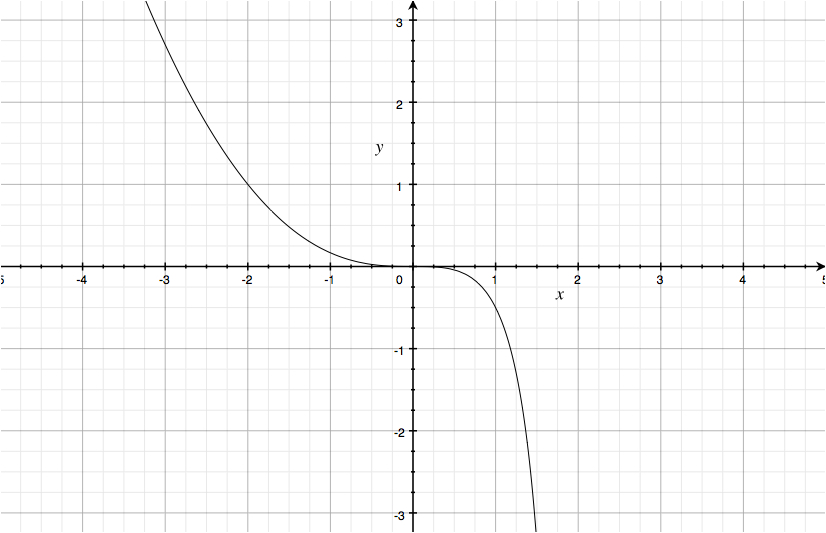
\includegraphics[scale=0.3]{../Figures/affineexample.jpg}
	\caption{The affine curve $x^3 - 2xy + 4y = 0$ in the visible part of $\an[2]$}
	\label{affinecurveexample}
\end{figure}

It is important to distinguish the two objects $V(f)$ and $f$, as $f$ is simply a polynomial, whereas $V(f)$ is the set of points that are a solution to a polynomial \emph{equation} $f(x_1,\ldots,x_n)=0$.
However, for convenience, we write the curve $V(f)$ as its defining polynomial equation $f(x_1,\ldots,x_n)=0$, when it is clear to do so, or even refer to just the curve $f$.
The distinction of objects remains, though, and this is purely notational.

More points on notation are that in the affine plane, instead of $x_1$ and $x_2$, we write $x$ and $y$, lowercase.
We also write polynomials as lowercase letters $f$, $g$ etc.
The reason for this will be explained shortly.
\subsubsection{Projective space}
Now that affine space has been introduced, we are ready to introduce projective $n$-space $\pn(k)$, and with that, the projective plane $\pn[2](k)$.

The projective plane is an idea that grew out of the renaissance study of perspective in art.
For example, when stood between two railway lines, they appear to meet at the horizon.
\Cref{projective-parallel} is a diagram of the situation.
While this is merely a trick of perspective in euclidean space, in the projective plane, parallel lines \emph{do} meet, at a so called `point at infinity'.
The idea is to add these points at infinity to the affine plane so that each line contains exactly one.
On top of this is the one exception, the `line at infinity', which is defined to be the unique line that is simply the collection of all points at infinity.
These ideas, while formative, are not rigorous, and we present the proper definition and constructions (there are two) of projective space below.

\begin{figure}[htbp]
	\centering
	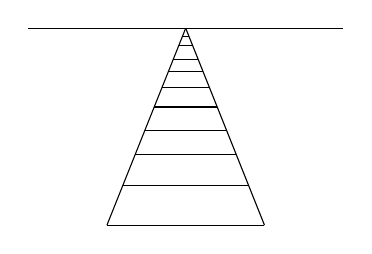
\begin{tikzpicture}[scale=0.5]
		% railway lines
		\draw (-2,0) -- (0,5);
		\draw (2,0) -- (0,5);
		% sleepers. To work out an appropriate x for given y, x=2(1-(y/5))
		\draw (-2,0) -- (2,0);
		\draw (-1.6,1) -- (1.6,1);
		\draw (-1.28,1.8) -- (1.28,1.8);
		\draw (-1.04,2.4) -- (1.04,2.4);
		\draw (-0.8,3) -- (0.8,3);
		\draw (-0.6,3.5) -- (0.6,3.5);
		\draw (-0.44,3.9) -- (0.44,3.9);
		\draw (-0.32,4.2) -- (0.32,4.2);
		\draw (-0.18,4.55) -- (0.18,4.55);
		\draw (-0.08,4.8) -- (0.08,4.8);
		% horizon
		\draw (-4,5) -- (4,5);
	\end{tikzpicture}
	\caption{Parallel lines `meeting' at infinity in euclidean space}
	\label{projective-parallel}
\end{figure}

The two constructions of projective space give two different interpretations of it, both of which are useful to consider.
Projective $n$-space can be thought of as either affine $n$-space with points at infinity added (mentioned already) or as a quotient of affine $(n+1)$-space.
For both of these constructions, $k$ is the underlying field of affine space $\an(k)$.

\subsubsection{Construction 1: Quotient of $\an[n+1](k)$}
Remove the origin (i.e. the point $(0,0,\ldots,0)$) from $\an[n+1](k)$ and define an equivalence relation $\sim$ on the remaining points as follows:
$$(a_0,a_1,\ldots,a_n) \sim (b_0,b_1,\ldots,b_n) \iff (a_0,a_1,\ldots,a_n) = \lambda(b_0,b_1,\ldots,b_n)$$
where $\lambda$ is a non-zero scalar in $\C$.
Then we have 
$$\pn = (\an[n+1](k)\setminus\{(0,\ldots,0)\})/\sim,$$
the set of equivalence classes of $\sim$.

Therefore, we see that points in $\pn$ are equivalence classes of lines in $\an[n+1](k) \setminus \{0\}$.
For points in $\pn$, write $P = [p_0,p_1,\ldots,p_n]$, where the square brackets represent the \emph{homogeneous coordinates} of the point.
We see that $[p_0,p_1,\ldots,p_n] = \{(\lambda p_0, \lambda p_1,\ldots,\lambda p_n) | \lambda \in \C, \lambda\neq0\}$.

By the nature of this construction, it is clear that scaling homogeneous coordinates results in coordinates of the same point.
Therefore, for a given point, there is no unique representation in homogeneous coordinates, and we may scale coordinates for our convenience.

\subsubsection{Construction 2: Extension of $\an[n](k)$}
Now we present the second construction of $\pn$, which can be thought of as adding points at infinity to affine $n$-space.
This is done inductively on $n$ by defining maps $\alpha_n$ and $\beta_n$.
To begin with, let $\pn[0] = \an[1](k) \setminus \{0\}$ and let
\begin{alignat*}{2}
	&\alpha_n : \an(k) \rightarrow \pn,\quad &&\alpha_n(x_1,\ldots,x_n) = [x_1,\ldots,x_n,1]\\
 &\beta_n : \pn[n-1] \rightarrow \pn,\quad &&\beta_n[X_1,\ldots,X_n] = [X_1,\ldots,X_n,0]
\end{alignat*}
Then we can define
$$\pn = \alpha_n(\an(k)) \cup \beta_n(\pn[n-1])$$
Effectively, we have that $\alpha_n$ is the embedding of affine space in $\pn$ and $\beta_n$ represents the points at infinity of $\pn$.
Notice that the image of $\beta_n$ will always give valid homogeneous coordinates, as we removed zero from $\pn[0]$, and therefore at least one of the first $n$ coordinates will be nonzero.
\subsubsection{Homogenisation and dehomogenisation}
Now that projective space has been introduced, we establish how to transition between affine space $\an$ and projective space $\pn$.
The second construction of projective space is the most enlightening in this regard.
The map $\alpha_n$ gives the image of a point $p=(x_1,\ldots,x_n)\in\an$ in $\pn$ as $[x_1,\ldots,x_n,1]$, and this process is known as \emph{homogenisation}.
From the first construction, which included the definition of homogeneous coordinates, we see that this can be scaled by any nonzero element of $k$, say $\lambda$, for example.
Then if we have homogeneous coordinates $[\lambda x_1,\ldots,\lambda x_n,\lambda]$, we can recover $p$ by dividing through by $\lambda$ (which is safe, since $\lambda\neq0$) such that the final homogeneous coordinate is 1, where we can recover the coordinates of the point from the first $n$ coordinates.
This transition from $\pn$ to $\an$ is known as \emph{dehomogenisation}, since it is the reverse transition to homogenisation.
More efficiently, to dehomogenise a point $P = [X_1,\ldots,X_n,X_{n+1}] \in \pn$ where $X_{n+1}\neq0$, we let $p = (\frac{X_1}{X_{n+1}},\ldots,\frac{X_n}{X_{n+1}})\in \an$.
Of course, the fact that we cannot dehomogenise points with final homogeneous coordinate 0 is to be expected, since these are the points at infinity, which do not exist in $\an$.

If we try to define projective curves in $\pn$ in the same way as affine curves, i.e. as solutions of a polynomial equation $f(x_1,\ldots,x_n)=0$ in $n$ variables, we find that it is not always possible, since we saw that the homogeneous coordinates of a point are not unique.
For example, if we tried to define a projective curve as $F(X,Y,Z)=X^2+Y+Z=0$, we see that $[2,-2,-2]$ is a solution of this equation, and so $[2,-2,-2] \in F$.
However, since we work with homogeneous coordinates, the point $[2,-2,-2]$ can also be written as $[-2,2,2]$, which clearly does not satisfy $F(X,Y,Z)=0$.
This is a problem, as we do not want the representation of a point to affect whether it lies on a curve or not.

To that extent, when working with the projective plane, it is convenient to define a homogeneous polynomial as a polynomial which satisfies
$$F(tX_1,tX_2,\ldots,tX_n)=t^e F(X_1,X_2,\ldots,X_n)$$
for some $t \in k$ and $e \in \N$.
We see that these kinds of polynomials are able to define curves in the projective plane, as for a homogeneous polynomial $F$,
$$F(X_1,X_2,\ldots,X_n)=0 \Leftrightarrow F(tX_1,tX_2,\ldots,tX_n) = t^k F(X_1,X_2,\ldots,X_n) = 0$$

It is easy enough to see that a polynomial is homogeneous if and only if the degree of each monomial $= d$, for some $d \in \N$.
So the polynomial $\frac{1}{2}x^4 + x^2y^2 + 14xy^3$ is homogeneous with degree 4, whereas the polynomial $17x^5 + 12x^2y + 2$ is not, as the monomials have degrees 5, 3 and 0, from left-to-right.

It is possible to homogenise a given polynomial $f(x_1,\ldots,x_n)$ by introducing another variable $x_{n+1}$ and multiplying each monomial by $x_{n+1}$ until it has degree $d$, where $d$ is the maximum degree of all monomials of $F$.
In practice, this resembles `topping up' the monomials with an extra variable as necessary.
So the inhomogeneous polynomial $17x^5 + 12x^2y + 2$ discussed earlier can be homogenised as $17X^5 + 12X^2YZ^2 + 2Z^5$.
The reverse transition can be made also, simply by letting $f = f(x_1,\ldots,x_n) = F(x_1,\ldots,x_n,1)$, which looks like simply taking out the extra variable.

When writing homogeneous polynomials, we use uppercase letters to distinguish them from affine variables and make the context clear.
We also use $X$, $Y$ and $Z$ (and also $x$ and $y$) as the three variables when dealing with the projective plane (uppercase) and the affine part thereof (lowercase).

To summarise, it is possible to move to (homogenisation) and from (dehomogenisation) the projective plane with regards to both points and polynomials.
A point $(x,y)\in\an[2]$ can be homogenised as $[x,y,1]\in\pn[2]$, and $[X,Y,Z]$ dehomogenised as $(X/Z,Y/Z)$.
A polynomial $f(x,y)$ can be homogenised as $F(X,Y,Z)$ by adding powers of $Z$ to each monomial as appropriate, and $F(X,Y,Z)$ dehomogenised as $f(x,y) = F(x,y,1)$.
\subsubsection{Projective curves and projective geometry}
Now that the concepts of homogenisation and dehomogenisation have been established, we introduce a few more ideas necessary for understanding the main subject matter.
From now on, we also limit ourselves to the projective plane $\pn[2]$.

\begin{definition}
	A projective curve is the set of points defined by a \emph{homogeneous} polynomial equation $F(X_1,X_2,\ldots,X_n) = 0$.
	When discussing the projective plane $\pn[2]$, we write $F(X,Y,Z) = 0$.
	The degree of a curve is the degree of the polynomial in the defining equation.
\end{definition}
For example, the polynomial equations $X^3-YZ^2=0$, $13X^2Z + Y^3 + 4XYZ = 0$ and $Z^2 + \frac{1}{2}Y^2 = 0$ all define projective curves in $\pn[2]$.
The first two have degree 3, the third, degree 2.

\begin{figure}[htbp]
	\centering
	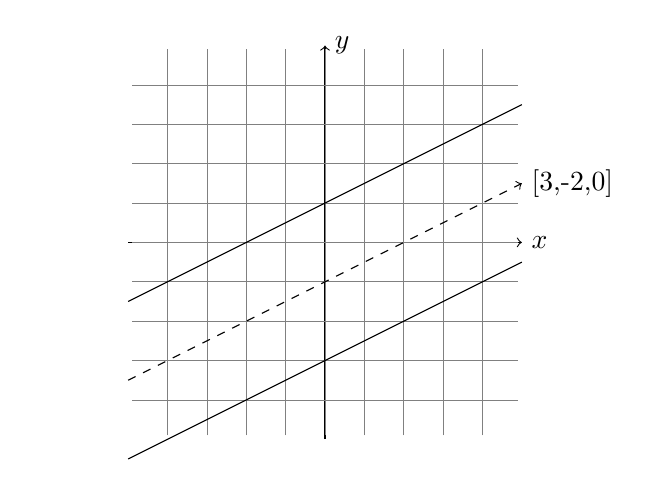
\begin{tikzpicture}[scale=0.5,domain=-5:5]
		% axes
		\draw[->] (-5,0) -- (5,0);
		\draw[->] (0,-5) -- (0,5);
		\node [right] at (5,0) {$x$};
		\node [right] at (0,5) {$y$};
		% grid
		\draw[help lines] (-4.9,-4.9) grid (4.9,4.9);
		% lines
		\draw 
		plot (\x, {0.5*\x+1});
		\draw 
		plot (\x, {0.5*\x-3});
		% annotation
		\draw[dashed,->]
		plot (\x, {0.5*\x-1});
		\node [right] at (5,1.5) {[3,-2,0]};
		\node [left,white] at (-5,1.5) {[3,-2,0]};
	\end{tikzpicture}
	\caption{The intersection of $2x - 3y + 1 = 0$ and $2x - 3y - 3 = 0$}
	\label{euclidean-intersection}
\end{figure}
While it is not possible to directly plot projective curves, as they contain points with complex coordinates and points at infinity in the projective plane, it is possible to see the affine part of projective curves $F$ by dehomogenising $F$ and looking at the resultant affine curve $f$.
The reverse is also true, and the parallel lines given by $2x - 3y + 1 = 0$ and $2x - 3y - 3 = 0$ in $\an[2]$ intersect in the projective plane at the point [3,-2,0].
This is because, when homogenised with respect to $Z$, the curves are given by $2X - 3Y + Z = 0$ and $2X - 3Y - 3Z = 0$, which are clearly satisfied by $[X,Y,Z] = [3,2,0]$.
As we would expect, this is a point at infinity, since $Z=0$.
This is illustrated in \cref{euclidean-intersection}.
\begin{definition}
	Let $F$ be a curve in $\pn[2]$ and $P=[a,b,c]$ be a point on $F$.
	Let $L$ be a line through $P$ with parametrisation
	$$\varphi(S,T) = SP + TQ = [Sa+Tu,Sb+Tv,Sc+Tw]$$
	for another point $Q$ on $L$.
	The \emph{intersection multiplicity} of $L$ and $F$ at $P$ is the multiplicity of $\varphi(1,0)$ as a solution of $F \circ \varphi = 0$, that is, the largest index $i$ such that $T^i$ is a factor of $F \circ \varphi = 0$
	The intersection is \emph{multiple} if the intersection multiplicity is greater than one, else it is \emph{regular}.
	\label{intersection-multiplicity}
\end{definition}
The concept of intersection multiplicity appears frequently in projective geometry, as we will see later.

We give an example of explicitly calculating the intersection multiplicity between the curve $F: YZ^2-X^3=0$ and the line $Y=0$ at the point $P = [0,0,1]$.
Let $Q = [1,0,1]$ such that $L$ has the parametrisation
$$L : [S,T] \mapsto [T,0,S+T].$$
Then $F(T,0,S+T) = 0 (S+T)^2 - T^3 = -T^3$, and since $T^3$ is a factor, the intersection has multiplicity 3.
\begin{definition}
	A singular point on a curve $F$ is a point $P$ where all partial derivatives $F_X$, $F_Y$ and $F_Z = 0$.
	An alternative characterisation is that the intersection multiplicity of a line and $F$ at $P$ is always greater than one.
	A point that is not a singular point is called a regular point.
\end{definition}
Two fundamental examples of projective curves with singular points are provided by the \emph{cusp} $C : Y^2Z - X^3$ and the \emph{node} $N : Y^2Z - X^3 - X^2Z$, which are illustrated in \cref{cuspandnode}.
\begin{figure}[htbp]
	\centering
	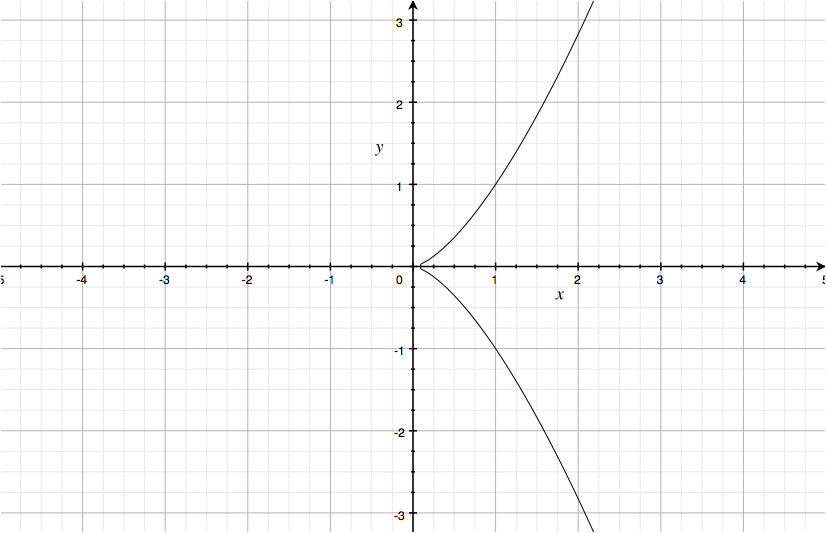
\includegraphics[scale=0.25]{../Figures/cusp.jpg}
	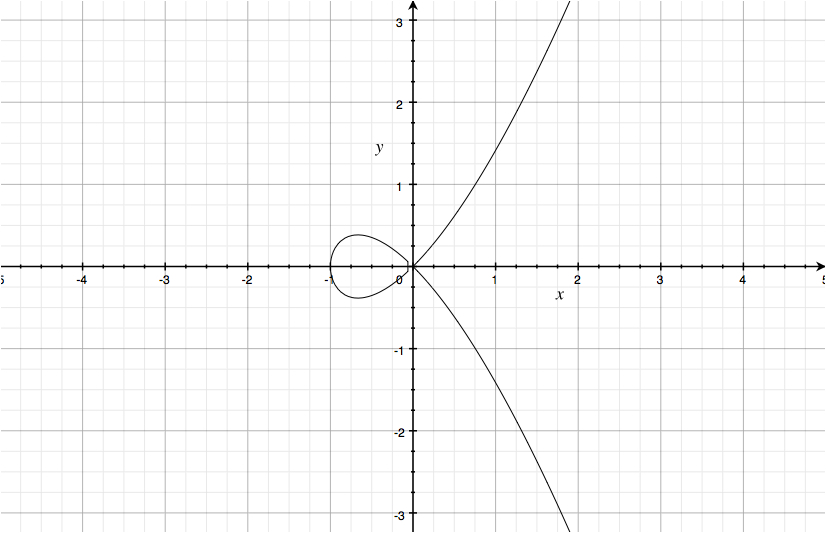
\includegraphics[scale=0.25]{../Figures/node.jpg}
	\caption{The cusp (left) and node (right) in the visible part of $\an[2]$}
	\label{cuspandnode}
\end{figure}
We can see that the point $[0,0,1]$ (the origin in the affine plane) is a singular point on both curves, since
\begin{alignat*}{2}
	&C_X = -3X^2,\qquad &&N_X = - 3X^2 - 2XZ\\
	&C_Y = 2YZ,\qquad &&N_Y = 2YZ\\
	&C_Z = Y^2,\qquad &&N_Z = Y^2 -X^2,
\end{alignat*}
and all partial derivatives vanish at $[0,0,1]$.

Singular points are important to consider as they are the points where there is no sensible notion of the tangent to a curve.
The importance of this will become apparent later on.

Supposing that a point on a curve is regular, and therefore has a tangent.
It is possible to find the equation of the line by examining the partial derivatives of the curve.
For example, let $F: X^3 - 3XZ^2 - Y^2Z = 0$ and consider the point $[0,1,0]$ on $F$.
We have $F_X(X,Y,Z) = 3X^2 -3Z^2$, $F_Y(X,Y,Z) = -2YZ$ and $F_Z(X,Y,Z) = -6XZ - Y^2$.
The equation of the tangent line $L$ is given by
$$L : F_X(P)X + F_Y(P)Y + F_Z(P)Z = 0$$
In this case, we have $L : -X - Z = 0$, or $L: X + Z = 0$.
As alluded to before, being able to find tangent lines plays an important part in our upcoming material.

\begin{definition}
	A curve that contains one or more singular points is a singular curve.
	Otherwise, the curve is regular.
\end{definition}

\begin{definition}
	A \emph{flex} is a point $P$ on a curve $F$ where the tangent to $F$ at $P$ intersects $F$ with multiplicity at least 3.
\end{definition}

The importance of flexes will become apparent in the next subsection.
Notice that the intersection of $F : Y^2Z - X^3 = 0$ and $Y=0$ that we calculated in \cref{intersection-multiplicity} is a flex of $F$, since it has intersection multiplicity 3.
\begin{definition}
	A projective transformation is a map $\pi : \pn[2] \rightarrow \pn[2]$ represented by a matrix
	$$\Pi = \left(
		\begin{matrix}
			\pi_{11} & \pi_{21} & \pi_{31}\\
			\pi_{12} & \pi_{22} & \pi_{32}\\
			\pi_{13} & \pi_{23} & \pi_{33}
		\end{matrix}
	\right).
	$$
\end{definition}
To find the image $P'$ of a point $P = [X,Y,Z]$ under the projective transformation $\pi$, we simply calculate $P' = \Pi [X,Y,Z]^{\mathrm{T}}$.
Since we work in the projective plane, and therefore homogeneous coordinates, two projective transformations $\pi$ and $\pi'$ are the same if and only if $\exists\lambda\in k$ such that $\Pi = \Pi'$.

We do not go into detail about projective transformations, but merely introduce them for their utility; the existence of projective transformations often allows simplifying assumptions to made about curves and points in the projective plane.
